\documentclass[12pt]{article}
\usepackage[utf8]{inputenc}
\usepackage{tgbonum}
\usepackage[a4paper, total={7in, 10in}]{geometry}
\usepackage{graphicx}
\usepackage{minted}
\title{Lab Assignment 4}
\author{Akshat Mittal - 20107}
\date{June 2021}
\begin{document}
\maketitle
\vspace{7mm}
\textbf{Contents}
\vspace{7mm}
\begin{enumerate}
    \item Dice Roll
    \item Seconds passed since last 12
    \item Fibonacci Series by recursion
    \item Currency Convertor
    \item Coin toss
    \item Guess the number
    \item Rounding off numbers
    \item Circular swapping
    \item Area of triangle and position of point
    \item Rectangular pattern
    \item Factorial using external header file
    \item Sum of the Series
\end{enumerate}

\newpage
\section{}
\subsection{Code}
\inputminted{c}{q1.c}
\subsection{Output}
\begin{figure}[h]
    \centering
    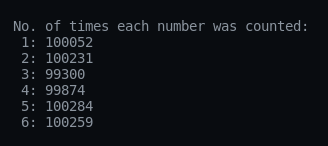
\includegraphics{1.png}
\end{figure}

\newpage
\section{}
\subsection{Code}
\inputminted{c}{q2.c}
\subsection{Output}
\begin{figure}[h]
    \centering
    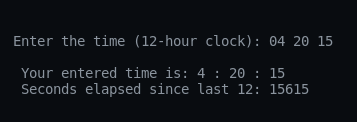
\includegraphics[width=0.5\textwidth]{2.png}
\end{figure}

\newpage
\section{}
\subsection{Code}
\inputminted{c}{q3.c}
\subsection{Output}
\begin{figure}[h]
    \centering
    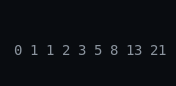
\includegraphics[width=0.5\textwidth]{3.png}
\end{figure}

\newpage
\section{}
\subsection{Code}
\inputminted{c}{q4.c}
\subsection{Output}
\begin{figure}[h]
    \centering
    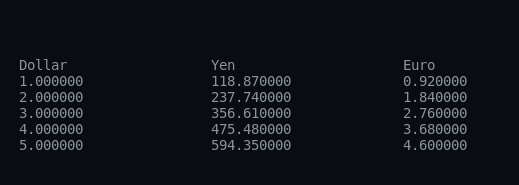
\includegraphics[width=0.9\textwidth]{4.png}
\end{figure}

\newpage
\section{}
\subsection{Code}
\inputminted{c}{q5.c}
\subsection{Output}
\begin{figure}[h]
    \centering
    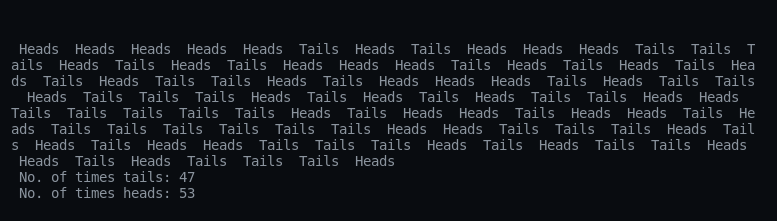
\includegraphics[width=1.0\textwidth]{5.png}
\end{figure}

\newpage
\section{}
\subsection{Code}
\inputminted{c}{q6.c}
\newpage
\subsection{Output}
\begin{figure}[h]
    \centering
    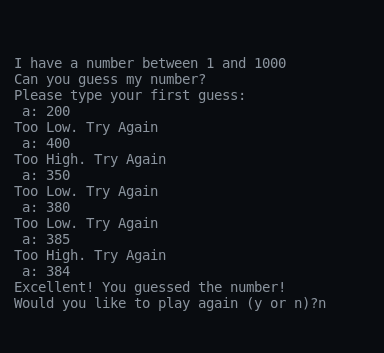
\includegraphics[width=0.75\textwidth]{6.png}
\end{figure}

\newpage
\section{}
\subsection{Code}
\inputminted{c}{q7.c}
\subsection{Output}
\begin{figure}[h]
    \centering
    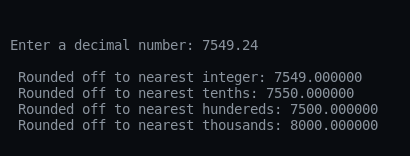
\includegraphics[width=0.75\textwidth]{7.png}
\end{figure}

\newpage
\section{}
\subsection{Code}
\inputminted{c}{q8.c}
\newpage
\subsection{Output}
\begin{figure}[h]
    \centering
    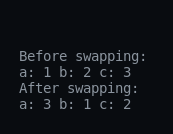
\includegraphics[width=0.5\textwidth]{8.png}
\end{figure}
\newpage
\section{}
\subsection{Code}
\inputminted{c}{q9.c}
\subsection{Output}
\begin{figure}[h]
    \centering
    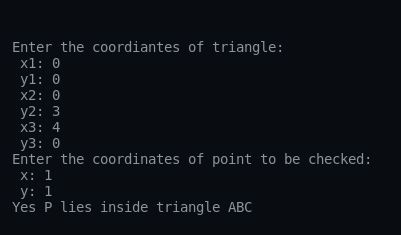
\includegraphics[width=0.7\textwidth]{9.png}
\end{figure}

\newpage
\section{}
\subsection{Code}
\inputminted{c}{q10.c}
\subsection{Output}
\begin{figure}[h]
    \centering
    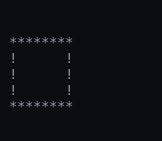
\includegraphics[width=0.8\textwidth]{10.png}
\end{figure}

\newpage
\section{}
\subsection{Code}
\inputminted{c}{q11.c}
\subsection{Output}
\begin{figure}[h]
    \centering
    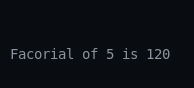
\includegraphics[width=0.8\textwidth]{11.png}
\end{figure}

\newpage
\section{}
\subsection{Code}
\inputminted{c}{q12.c}
\subsection{Output}
\begin{figure}[h]
    \centering
    
\includegraphics[width=0.8\textwidth]{12.png}
\end{figure}

\end{document}